\documentclass[11pt,a4paper]{article}
\usepackage{fontspec}
\setmainfont[Path=fonts/,FontIndex=7,BoldFont=AvenirNext.ttc,BoldFeatures={FontIndex=2},ItalicFont=AvenirNext.ttc,ItalicFeatures={FontIndex=4},BoldItalicFont=AvenirNext.ttc,BoldItalicFeatures={FontIndex=3}]{AvenirNext.ttc}
\setsansfont[Path=fonts/,FontIndex=7,BoldFont=AvenirNext.ttc,BoldFeatures={FontIndex=2},ItalicFont=AvenirNext.ttc,ItalicFeatures={FontIndex=4},BoldItalicFont=AvenirNext.ttc,BoldItalicFeatures={FontIndex=3}]{AvenirNext.ttc}
\newfontfamily\heavy[Path=fonts/,FontIndex=2]{AvenirNext.ttc}
\setmonofont[Path=fonts/,BoldFont=JetBrainsMono-Bold.ttf,ItalicFont=JetBrainsMono-Italic.ttf,Contextuals=NoAlternate,Ligatures=NoCommon]{JetBrainsMono-Regular.ttf}
\usepackage{xcolor,graphicx,tikz,booktabs,tabularx,listings,amsmath}
\usetikzlibrary{arrows.meta,positioning}
\definecolor{paper}{HTML}{FFFFFF}
\definecolor{ink}{HTML}{252525}
\definecolor{teal}{HTML}{252525}
\definecolor{orange}{HTML}{777777}
\definecolor{wash}{HTML}{EAEAEA}
\definecolor{quiet}{HTML}{666666}
\definecolor{lightink}{HTML}{D0D0D0}
\definecolor{codepaper}{HTML}{F6F6F4}
\lstset{language=Python,basicstyle=\ttfamily\fontsize{9.5}{13}\selectfont\color{ink},keywordstyle=\bfseries\color{ink},commentstyle=\itshape\color{quiet},stringstyle=\color{ink},showstringspaces=false,columns=fullflexible,keepspaces=true,breaklines=true,breakatwhitespace=true,numbers=none,upquote=true,aboveskip=8pt,belowskip=6pt}
\hyphenpenalty=4000
\emergencystretch=3em
% The same two-line navigation and fine rule as the reference, without a candy motif.
\newcommand{\guideheader}[2]{\begin{tikzpicture}[remember picture,overlay]
\node[anchor=north west,inner sep=0,text width=176mm] at ([xshift=16mm,yshift=-7mm]current page.north west) {\fontsize{8.5}{10}\selectfont\color{quiet}#1};
\node[anchor=north west,inner sep=0,text width=176mm] at ([xshift=16mm,yshift=-11.5mm]current page.north west) {\heavy\fontsize{10}{12}\selectfont\color{ink}#2};
\draw[lightink,line width=.4pt] ([xshift=16mm,yshift=-17mm]current page.north west)--([xshift=192mm,yshift=-17mm]current page.north west);
\end{tikzpicture}}

\usepackage[a4paper,left=16mm,right=18mm,top=24mm,bottom=19mm,headheight=14pt]{geometry}
\usepackage{fancyhdr,enumitem,hyperref}
\hypersetup{colorlinks=true,linkcolor=teal,urlcolor=teal}
\setlength{\parindent}{0pt}
\setlength{\parskip}{7pt}
\setlist{nosep,leftmargin=1.4em}
\usepackage{needspace,colortbl}
\lstdefinestyle{numbered}{numbers=left,numberstyle=\ttfamily\fontsize{7.5}{13}\selectfont\color{lightink},numbersep=10pt,xleftmargin=24pt}
\pagestyle{fancy}\fancyhf{}
\fancyhead[C]{\guideheader{Lesson 4 · Fruit Feast}{Worksheet Answers · \nouppercase{\leftmark}}}
\fancyfoot[L]{\fontsize{8}{10}\selectfont\color{quiet}LESSON 4 / Fruit Feast}
\fancyfoot[R]{\fontsize{9}{11}\selectfont\color{quiet}\thepage}
\renewcommand{\headrulewidth}{0pt}
\newcommand{\topic}[2]{\clearpage\markboth{#2}{}{\color{quiet}\fontsize{9}{12}\selectfont\textbf{#1}}\par{\heavy\fontsize{19}{23}\selectfont\raggedright #2\par}\vspace{5pt}}
\newcommand{\topicflow}[2]{\par\Needspace{20\baselineskip}\bigskip\markboth{#2}{}{\color{quiet}\fontsize{9}{12}\selectfont\textbf{#1}}\par{\heavy\fontsize{19}{23}\selectfont\raggedright #2\par}\vspace{5pt}}
\newcommand{\labeltext}[1]{{\color{teal}\textbf{#1}}\par}
\makeatletter
\newsavebox{\qbox}
\newenvironment{qblock}[1][0.6]{\def\qlimit{#1}\par\setbox\qbox\vbox\bgroup\hsize\linewidth\color@begingroup}{\par\color@endgroup\egroup
  \ifdim\dimexpr\ht\qbox+\dp\qbox\relax>\qlimit\textheight\relax\unvbox\qbox\else\box\qbox\fi\par}
\makeatother
\newcommand{\qtopic}[2]{{\color{quiet}\fontsize{9}{12}\selectfont\textbf{#1}}\par{\heavy\fontsize{19}{23}\selectfont\raggedright #2\par}\vspace{5pt}}
\begin{document}\color{ink}\fontsize{10.5}{13}\selectfont
\thispagestyle{empty}\pagecolor{white}\null
\begin{tikzpicture}[remember picture,overlay]
\node[anchor=north west,inner sep=0,text width=174mm] at ([xshift=18mm,yshift=-22mm]current page.north west)
{\heavy\fontsize{9}{12}\selectfont ALGORITHMS\quad /\quad LESSON 04\quad /\quad WORKSHEET ANSWERS};
\node[anchor=north west,inner sep=0,text width=174mm] at ([xshift=18mm,yshift=-39mm]current page.north west)
{\heavy\fontsize{43}{47}\selectfont\raggedright\spaceskip=.25em Fruit\\Feast\par};
\node[anchor=north west,inner sep=0,text width=174mm] at ([xshift=18mm,yshift=-80mm]current page.north west)
{\fontsize{19}{25}\selectfont Worked answers, tables and complete code.};
\node[anchor=north west,inner sep=0,text width=150mm] at ([xshift=18mm,yshift=-97mm]current page.north west)
{\fontsize{12}{16}\selectfont Check each answer against your own working.\\Follow the question IDs from the worksheet.};
\node[anchor=center,inner sep=0] at ([xshift=105mm,yshift=-167mm]current page.north west)
{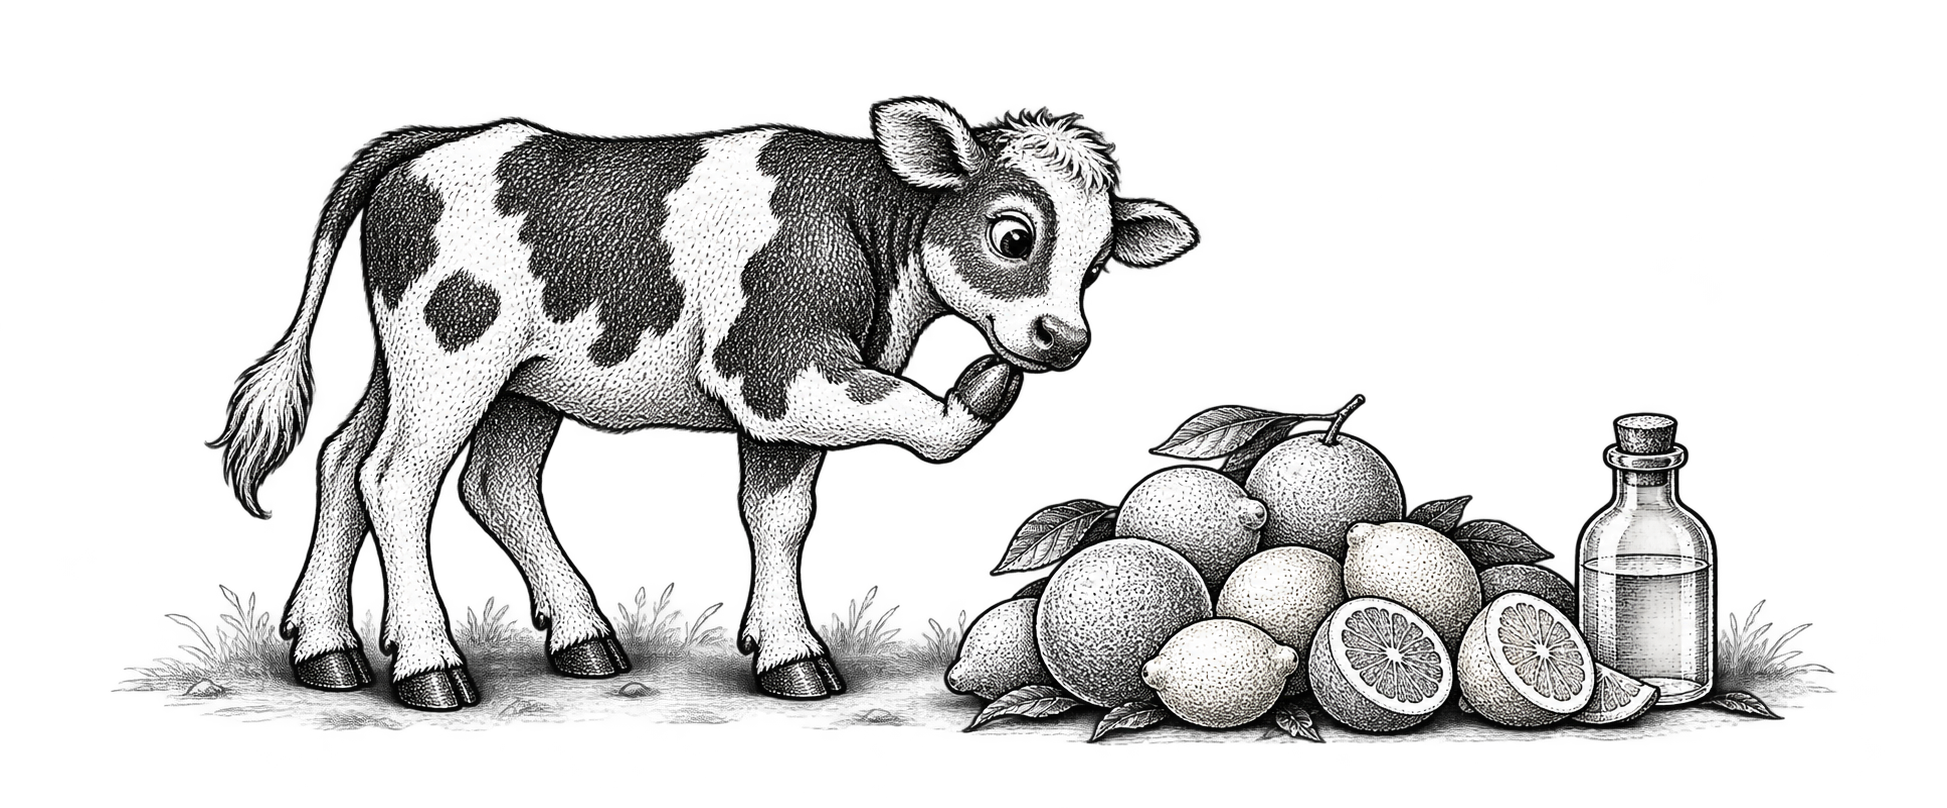
\includegraphics[width=174mm,height=94mm,keepaspectratio]{assets/cover.png}};
\node[anchor=north west,inner sep=0,text width=174mm] at ([xshift=18mm,yshift=-224mm]current page.north west)
{\fontsize{12}{16}\selectfont Questions appear in worksheet order.\\Alternative correct solutions are welcome.};
\node[anchor=west,inner sep=0] at ([xshift=18mm,yshift=-269mm]current page.north west)
{
\includegraphics[width=43mm]{assets/logo.png}};
\node[anchor=east,inner sep=0] at ([xshift=192mm,yshift=-269mm]current page.north west)
{
\includegraphics[width=62mm]{assets/julians-pathfinder-monochrome.pdf}};
\end{tikzpicture}\clearpage
\topic{KEEP BESIDE YOUR WORK}{The route and the rules}
\textbf{Our route}\par First find all fullness values reachable without water. Next consider drinking from each of those values. Finally add fruit after the drink. Keep these three lists of results separate while tracing the example; they represent different moments in the calculation.\par\medskip
\textbf{Fruit Feast rules}\par The cow starts with fullness 0. There is unlimited fruit: one type adds a and the other adds b, both positive integers. Fullness must never exceed limit. A fruit that would exceed limit cannot be eaten. The cow may stop at any time; find the largest fullness she can reach.\par\medskip
\textbf{The one drink}\par Water is optional and can be used at most once, before, between or after eating. It changes fullness f to \texttt{f // 2}, where // rounds down. For example, 5 becomes 2. Fruit may be eaten afterwards, but a second drink is forbidden.\par\medskip
\textbf{Names used in the questions}\par \texttt{dry[f]} says whether fullness f is reachable without having used water. \texttt{wet[f]} says whether it is reachable after using water. The position f is a fullness value. The entry is a yes/no flag, not a count of routes. Write Y for reachable and - for unreachable in the printed tables.\par\medskip
\textbf{Recursion and the table answer different questions}\par The recursive function returns the largest final fullness reachable from the current situation. The iterative tables store which situations can be reached from the start. Both must obey the same fruit and water rules. When tracing, always label which kind of answer you are recording.\par\medskip
\textbf{Using these answers.} Each question and its supplied diagram or table appear before the answer. Completed tables, and answer diagrams where the question has one, follow the worked answer. The IDs match the worksheet; answer pages have their own page numbers. Each program is printed in full once, with imports, line numbers and a small check; a later question that uses the same program names the page where it appears and gives its own check.\par\bigskip{\color{lightink}\hrule height .4pt}\bigskip\par\markboth{Eating without going over}{}\begin{qblock}\begin{qblock}[0.95]
\qtopic{L4-01}{Eating without going over}
{\small\color{quiet}Understand the fruit and water choices}\par\medskip
\textbf{Question.} Fullness starts at 0 and must never exceed 10. An orange adds 4 and a lemon adds 7. You may eat either fruit repeatedly. Without water, what fullness values are reachable?

\par\medskip\textbf{Worked answer.} The reachable values are 0, 4, 7 and 8. The best is 8. Eating 4 then 7 would reach 11, so that action is forbidden rather than clipped back to 10.

\end{qblock}
\end{qblock}\par\medskip{\color{lightink}\hrule height .4pt}\bigskip
\par\markboth{Water can make room}{}\begin{qblock}\begin{qblock}[0.95]
\qtopic{L4-02}{Water can make room}
{\small\color{quiet}Understand the fruit and water choices}\par\medskip
\textbf{Question.} At most once, the cow may drink water. Water halves the current fullness, rounding down. With limit 10 and fruit sizes 4 and 7, find a route to fullness 10.

\par\medskip\textbf{Worked answer.} Eat a lemon: 0 to 7. Drink: 7 // 2 = 3. Eat another lemon: 3 to 10. This reaches the limit exactly, so no better answer is possible.

\textbf{Diagram for the answer.}\par\begin{center}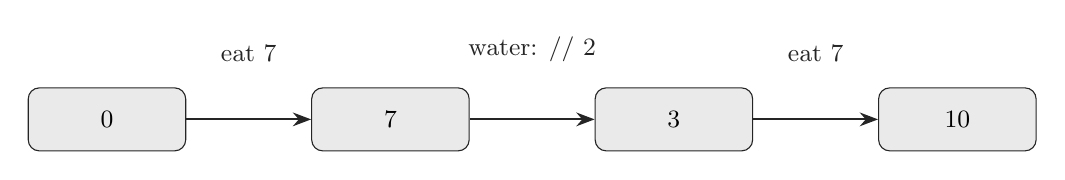
\begin{tikzpicture}[>=Stealth,every node/.style={font=\small},box/.style={draw=teal,rounded corners,minimum width=20mm,minimum height=8mm,fill=wash},arr/.style={->,thick,teal}]\node[box] (p0) at (0.0,0) {0};\node[box] (p1) at (3.6,0) {7};\node[box] (p2) at (7.2,0) {3};\node[box] (p3) at (10.8,0) {10};\draw[arr] (p0)--node[above=6mm]{eat 7}(p1);\draw[arr] (p1)--node[above=6mm]{water: // 2}(p2);\draw[arr] (p2)--node[above=6mm]{eat 7}(p3);\end{tikzpicture}\end{center}
\end{qblock}
\end{qblock}\par\medskip{\color{lightink}\hrule height .4pt}\bigskip
\par\markboth{Same fullness, different choices}{}\begin{qblock}\begin{qblock}[0.95]
\qtopic{L4-03}{Same fullness, different choices}
{\small\color{quiet}Understand the fruit and water choices}\par\medskip
\textbf{Question.} A reachability flag is a yes/no answer: can the cow reach this situation? Compare fullness 4 with water still unused and fullness 4 after drinking. Do they allow the same next actions? Why would one flag called reachable[4] lose information we need?

\par\medskip\textbf{Worked answer.} No. Before water, drinking is still available. After water, it is forbidden. Use dry[4] for reachable without drinking and wet[4] for reachable after drinking.

For example, from fullness 4 with water unused, drinking can move to fullness 2. From fullness 4 with water already used, that move is illegal. A single flag would hide whether this next action is allowed.

\end{qblock}
\end{qblock}\par\medskip{\color{lightink}\hrule height .4pt}\bigskip
\par\markboth{A small recursive search}{}\begin{qblock}\begin{qblock}[0.95]
\qtopic{L4-04}{A small recursive search}
{\small\color{quiet}Understand the fruit and water choices}\par\medskip
\textbf{Question.} Write feast\_cached(limit, a, b) using cached recursion. The helper asks: from fullness f, with used\_water saying whether the drink has been used, what is the greatest final fullness reachable? List every legal next action, including stopping. Explain why f and used\_water belong in the cache key.

\par\smallskip{\small\textbf{Start with:}}\par\smallskip\noindent\colorbox{codepaper}{\parbox{\dimexpr\linewidth-2\fboxsep\relax}{\small\ttfamily\raggedright def feast\_cached(limit, a, b):\\\hspace*{2.4em}def best(fullness, used\_water):\\\hspace*{4.8em}return None  \# Your helper goes here.\\\hspace*{2.4em}return best(0, False)}}\par
{\small\textbf{What each function returns.}\par feast\_cached(limit, a, b): the greatest reachable fullness, starting empty with water unused.\par best(fullness, used\_water): the greatest final fullness reachable from this fullness and water status.\par }
{\small\textbf{Hints.}}\begin{itemize}\item Stopping is always allowed. What does that give as a first answer?\item Which moves are legal from (fullness, used\_water)?\item Which move changes used\_water, and can it happen twice?\end{itemize}
\par\medskip\textbf{Worked answer.} Try either fruit if it fits, and water only if it is unused. Also allow stopping at the current fullness. Cache the best final fullness for each pair. The same fullness with a different water status has different legal futures.

Stopping returns the current fullness f, so the cow is never forced to make another move. Eating keeps the water status unchanged. Drinking changes the status from unused to used, even at fullness 0; it cannot create a cycle back to an unused-water state.

\end{qblock}
\begin{qblock}[0.95]
\medskip\textbf{One complete Python implementation: feast\_cached.}\label{ans-feast_cached}\par
\begin{lstlisting}[style=numbered]
from functools import lru_cache

def feast_cached(limit, a, b):
    @lru_cache(None)
    def best(fullness, used_water):
        answer = fullness
        for fruit in (a, b):
            if fullness + fruit <= limit:
                answer = max(answer, best(fullness + fruit, used_water))
        if not used_water:
            answer = max(answer, best(fullness // 2, True))
        return answer
    return best(0, False)
\end{lstlisting}
\textbf{Check.} Run this after the function above.
\begin{lstlisting}
print(feast_cached(10, 4, 7))
\end{lstlisting}
\textbf{Expected output.}
\begin{lstlisting}[language={}]
10
\end{lstlisting}
\textbf{Recursion depth.} Python stops recursion at about 1,000 nested calls by default, so this recursive version is for small inputs and the small and edge test files only. Use the iterative version for the medium and large files.

\end{qblock}
\end{qblock}\par\medskip{\color{lightink}\hrule height .4pt}\bigskip
\par\markboth{First, all fullness values before water}{}\begin{qblock}\begin{qblock}[0.95]
\qtopic{L4-05}{First, all fullness values before water}
{\small\color{quiet}Build the three passes}\par\medskip
\textbf{Question.} For limit 10 and fruit sizes 4 and 7, fill dry[0] through dry[10]. Why can the scan run from low fullness to high fullness?

\textbf{Table supplied with the question.}\par\par\medskip \begingroup\footnotesize\setlength{\tabcolsep}{4pt}\renewcommand{\arraystretch}{1.35}\begin{tabularx}{\linewidth}{>{\raggedright\arraybackslash}l>{\raggedright\arraybackslash}X>{\raggedright\arraybackslash}X>{\raggedright\arraybackslash}X>{\raggedright\arraybackslash}X>{\raggedright\arraybackslash}X>{\raggedright\arraybackslash}X>{\raggedright\arraybackslash}X>{\raggedright\arraybackslash}X>{\raggedright\arraybackslash}X>{\raggedright\arraybackslash}X>{\raggedright\arraybackslash}X}\toprule\textbf{Fullness f} & \textbf{0} & \textbf{1} & \textbf{2} & \textbf{3} & \textbf{4} & \textbf{5} & \textbf{6} & \textbf{7} & \textbf{8} & \textbf{9} & \textbf{10}\\\midrule
dry[f] & Y & ? & ? & ? & ? & ? & ? & ? & ? & ? & ?\\
\bottomrule\end{tabularx}\endgroup\par\medskip 
\par\medskip\textbf{Worked answer.} Only dry[0], dry[4], dry[7] and dry[8] are true. Fruit adds a positive amount, so it always moves to a larger index. A forward scan reaches those new states later.

\textbf{Completed table.}\par\par\medskip \begingroup\footnotesize\setlength{\tabcolsep}{4pt}\renewcommand{\arraystretch}{1.35}\begin{tabularx}{\linewidth}{>{\raggedright\arraybackslash}l>{\raggedright\arraybackslash}X>{\raggedright\arraybackslash}X>{\raggedright\arraybackslash}X>{\raggedright\arraybackslash}X>{\raggedright\arraybackslash}X>{\raggedright\arraybackslash}X>{\raggedright\arraybackslash}X>{\raggedright\arraybackslash}X>{\raggedright\arraybackslash}X>{\raggedright\arraybackslash}X>{\raggedright\arraybackslash}X}\toprule\textbf{Fullness f} & \textbf{0} & \textbf{1} & \textbf{2} & \textbf{3} & \textbf{4} & \textbf{5} & \textbf{6} & \textbf{7} & \textbf{8} & \textbf{9} & \textbf{10}\\\midrule
dry[f] & Y & - & - & - & Y & - & - & Y & Y & - & -\\
\bottomrule\end{tabularx}\endgroup\par\medskip 
\end{qblock}
\end{qblock}\par\medskip{\color{lightink}\hrule height .4pt}\bigskip
\par\markboth{Then, drink from every dry state}{}\begin{qblock}\begin{qblock}[0.95]
\qtopic{L4-06}{Then, drink from every dry state}
{\small\color{quiet}Build the three passes}\par\medskip
\textbf{Question.} Take every fullness you marked as reachable without water in L4-05. Halve each one, rounding down, to find the states immediately after drinking and before any further fruit. Why would drinking only from the largest dry value miss a useful possibility?

\par\medskip\textbf{Worked answer.} The immediate-after-water values are 0, 2, 3 and 4: halve 0, 4, 7 and 8 respectively. Drinking at fullness 7 gives 3, then eating a fruit of size 7 reaches 10. Drinking only at fullness 8 gives 4, from which the largest reachable value is 8. It misses the best route.

\textbf{Diagram for the answer.}\par\begin{center}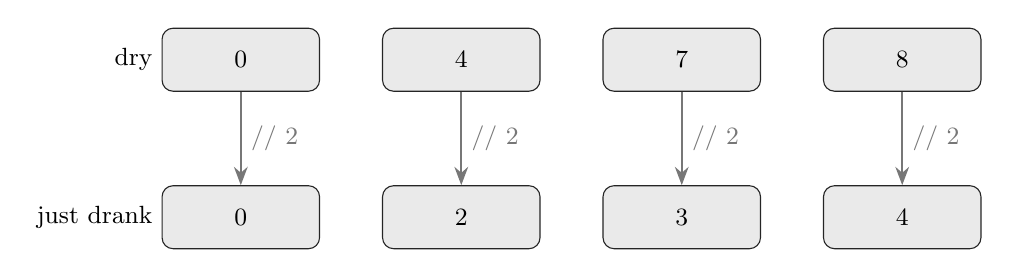
\begin{tikzpicture}[>=Stealth,every node/.style={font=\small},box/.style={draw=teal,rounded corners,minimum width=20mm,minimum height=8mm,fill=wash},arr/.style={->,thick,teal}]\node[anchor=east] at (-1,0) {dry};\node[anchor=east] at (-1,-2) {just drank};\node[box] (a0) at (0.0,0) {0};\node[box] (b0) at (0.0,-2) {0};\draw[arr,orange] (a0)--node[right]{// 2}(b0);\node[box] (a1) at (2.8,0) {4};\node[box] (b1) at (2.8,-2) {2};\draw[arr,orange] (a1)--node[right]{// 2}(b1);\node[box] (a2) at (5.6,0) {7};\node[box] (b2) at (5.6,-2) {3};\draw[arr,orange] (a2)--node[right]{// 2}(b2);\node[box] (a3) at (8.399999999999999,0) {8};\node[box] (b3) at (8.399999999999999,-2) {4};\draw[arr,orange] (a3)--node[right]{// 2}(b3);\end{tikzpicture}\end{center}
\end{qblock}
\end{qblock}\par\medskip{\color{lightink}\hrule height .4pt}\bigskip
\par\markboth{Finally, eat after water}{}\begin{qblock}\begin{qblock}[0.95]
\qtopic{L4-07}{Finally, eat after water}
{\small\color{quiet}Build the three passes}\par\medskip
\textbf{Question.} Start from the values you found in L4-06 immediately after drinking. Fruit adds 4 or 7 and the limit is 10. Mark every fullness reachable after any further fruit, including no further fruit. A second drink is forbidden. What is the largest reachable fullness?

\textbf{Table supplied with the question.}\par\par\medskip \begingroup\footnotesize\setlength{\tabcolsep}{4pt}\renewcommand{\arraystretch}{1.35}\begin{tabularx}{\linewidth}{>{\raggedright\arraybackslash}l>{\raggedright\arraybackslash}X>{\raggedright\arraybackslash}X>{\raggedright\arraybackslash}X>{\raggedright\arraybackslash}X>{\raggedright\arraybackslash}X>{\raggedright\arraybackslash}X>{\raggedright\arraybackslash}X>{\raggedright\arraybackslash}X>{\raggedright\arraybackslash}X>{\raggedright\arraybackslash}X>{\raggedright\arraybackslash}X}\toprule\textbf{Fullness f} & \textbf{0} & \textbf{1} & \textbf{2} & \textbf{3} & \textbf{4} & \textbf{5} & \textbf{6} & \textbf{7} & \textbf{8} & \textbf{9} & \textbf{10}\\\midrule
wet[f] &  &  &  &  &  &  &  &  &  &  & \\
\bottomrule\end{tabularx}\endgroup\par\medskip 
\par\medskip\textbf{Worked answer.} The wet states are 0, 2, 3, 4, 6, 7, 8, 9 and 10. The largest reachable fullness in either layer is 10. No water transition is allowed from the wet layer.

\textbf{Completed table.}\par\par\medskip \begingroup\footnotesize\setlength{\tabcolsep}{4pt}\renewcommand{\arraystretch}{1.35}\begin{tabularx}{\linewidth}{>{\raggedright\arraybackslash}l>{\raggedright\arraybackslash}X>{\raggedright\arraybackslash}X>{\raggedright\arraybackslash}X>{\raggedright\arraybackslash}X>{\raggedright\arraybackslash}X>{\raggedright\arraybackslash}X>{\raggedright\arraybackslash}X>{\raggedright\arraybackslash}X>{\raggedright\arraybackslash}X>{\raggedright\arraybackslash}X>{\raggedright\arraybackslash}X}\toprule\textbf{Fullness f} & \textbf{0} & \textbf{1} & \textbf{2} & \textbf{3} & \textbf{4} & \textbf{5} & \textbf{6} & \textbf{7} & \textbf{8} & \textbf{9} & \textbf{10}\\\midrule
wet[f] & Y & - & Y & Y & Y & - & Y & Y & Y & Y & Y\\
\bottomrule\end{tabularx}\endgroup\par\medskip 
Starting from the immediate-after-water values 0, 2, 3 and 4: 0 can reach 4, 7 and 8; 2 can reach 6, 9 and 10; 3 can reach 7 and 10; 4 can reach 8. Include the starting values too because eating no further fruit is allowed.

\end{qblock}
\end{qblock}\par\medskip{\color{lightink}\hrule height .4pt}\bigskip
\par\markboth{The complete three-pass program}{}\begin{qblock}\begin{qblock}[0.95]
\qtopic{L4-08}{The complete three-pass program}
{\small\color{quiet}Build the three passes}\par\medskip
\textbf{Question.} Write feast\_table(limit, a, b) with three passes: eat before water, drink once from each reachable value, then eat after water. A bytearray is a compact list of integers, initially all 0. Use 1 for reachable states. Explain the two arrays, scan order and choice of final answer.

\par\smallskip{\small\textbf{Start with:}}\par\smallskip\noindent\colorbox{codepaper}{\parbox{\dimexpr\linewidth-2\fboxsep\relax}{\small\ttfamily\raggedright def feast\_table(limit, a, b):\\\hspace*{2.4em}return None  \# Replace with your answer.}}\par
{\small\textbf{What each function returns.}\par feast\_table(limit, a, b): the greatest reachable fullness, starting empty with water unused.\par }
{\small\textbf{Hints.}}\begin{itemize}\item Which fullness is reachable before anything is eaten?\item Keep the three passes in order: eat, drink once, eat again.\item Which array does each pass read, and which does it write?\end{itemize}
\par\medskip\textbf{Worked answer.} dry[f] and wet[f] are yes/no flags for fullness f before and after using water. Mark dry[0], complete dry by adding fruit, set wet[f // 2] for every reachable dry f, then complete wet by adding fruit. Return the largest f marked in either array. Three passes and one final search take O(limit) time and memory.

\end{qblock}
\begin{qblock}[0.95]
\medskip\textbf{One complete Python implementation: feast\_table.}\label{ans-feast_table}\par
\begin{lstlisting}[style=numbered]
def feast_table(limit, a, b):
    dry = bytearray(limit + 1)
    wet = bytearray(limit + 1)
    dry[0] = 1
    for fullness in range(limit + 1):
        if dry[fullness]:
            for fruit in (a, b):
                if fullness + fruit <= limit:
                    dry[fullness + fruit] = 1
    for fullness in range(limit + 1):
        if dry[fullness]:
            wet[fullness // 2] = 1
    for fullness in range(limit + 1):
        if wet[fullness]:
            for fruit in (a, b):
                if fullness + fruit <= limit:
                    wet[fullness + fruit] = 1
    for fullness in range(limit, -1, -1):
        if dry[fullness] or wet[fullness]:
            return fullness
\end{lstlisting}
\textbf{Check.} Run this after the function above.
\begin{lstlisting}
print(feast_table(10, 4, 7))
\end{lstlisting}
\textbf{Expected output.}
\begin{lstlisting}[language={}]
10
\end{lstlisting}
\end{qblock}
\end{qblock}\par\medskip{\color{lightink}\hrule height .4pt}\bigskip
\par\markboth{Your turn: a different feast}{}\begin{qblock}\begin{qblock}[0.95]
\qtopic{L4-09}{Your turn: a different feast}
{\small\color{quiet}Test and explain the pass order}\par\medskip
\textbf{Question.} Use limit 9 and fruit sizes 4 and 6. Mark three rows: reachable without water; immediately after drinking; after any further fruit. Keep the water-only row separate from the completed wet row. Give a route to the largest final fullness. Test your feast\_table(limit, a, b) from L4-08 on this example.

\textbf{Table supplied with the question.}\par\par\medskip \begingroup\footnotesize\setlength{\tabcolsep}{4pt}\renewcommand{\arraystretch}{1.35}\begin{tabularx}{\linewidth}{>{\raggedright\arraybackslash}l>{\raggedright\arraybackslash}X>{\raggedright\arraybackslash}X>{\raggedright\arraybackslash}X>{\raggedright\arraybackslash}X>{\raggedright\arraybackslash}X>{\raggedright\arraybackslash}X>{\raggedright\arraybackslash}X>{\raggedright\arraybackslash}X>{\raggedright\arraybackslash}X>{\raggedright\arraybackslash}X}\toprule\textbf{Fullness f} & \textbf{0} & \textbf{1} & \textbf{2} & \textbf{3} & \textbf{4} & \textbf{5} & \textbf{6} & \textbf{7} & \textbf{8} & \textbf{9}\\\midrule
dry[f] & Y &  &  &  &  &  &  &  &  & \\
just drank &  &  &  &  &  &  &  &  &  & \\
wet[f] &  &  &  &  &  &  &  &  &  & \\
\bottomrule\end{tabularx}\endgroup\par\medskip 
\par\medskip\textbf{Worked answer.} Dry: 0, 4, 6, 8. Immediately after water: 0, 2, 3, 4. After further fruit: 0, 2, 3, 4, 6, 7, 8, 9. Best: 9, using 0 to 6, drink to 3, then add 6.

\textbf{Completed table.}\par\par\medskip \begingroup\footnotesize\setlength{\tabcolsep}{4pt}\renewcommand{\arraystretch}{1.35}\begin{tabularx}{\linewidth}{>{\raggedright\arraybackslash}l>{\raggedright\arraybackslash}X>{\raggedright\arraybackslash}X>{\raggedright\arraybackslash}X>{\raggedright\arraybackslash}X>{\raggedright\arraybackslash}X>{\raggedright\arraybackslash}X>{\raggedright\arraybackslash}X>{\raggedright\arraybackslash}X>{\raggedright\arraybackslash}X>{\raggedright\arraybackslash}X}\toprule\textbf{Fullness f} & \textbf{0} & \textbf{1} & \textbf{2} & \textbf{3} & \textbf{4} & \textbf{5} & \textbf{6} & \textbf{7} & \textbf{8} & \textbf{9}\\\midrule
dry[f] & Y & - & - & - & Y & - & Y & - & Y & -\\
just drank & Y & - & Y & Y & Y & - & - & - & - & -\\
wet[f] & Y & - & Y & Y & Y & - & Y & Y & Y & Y\\
\bottomrule\end{tabularx}\endgroup\par\medskip 
The final row also keeps every value in the just-drank row. From fullness 2, further fruit reaches 6 or 8. From fullness 3, it reaches 7 or 9. No continuation reaches fullness 5, so that entry remains unmarked.

\end{qblock}
\end{qblock}\par\medskip{\color{lightink}\hrule height .4pt}\bigskip
\par\markboth{Boundary tests and optional water}{}\begin{qblock}\begin{qblock}[0.95]
\qtopic{L4-10}{Boundary tests and optional water}
{\small\color{quiet}Test and explain the pass order}\par\medskip
\textbf{Question.} Test your feast\_table(limit, a, b) from L4-08. Here limit is maximum fullness, and a and b are the fruit increases. First predict the answers for (1, 1, 1), (8, 4, 6) and (5, 4, 4), then run your function. Must the cow drink? Give a route for each answer.

\par\medskip\textbf{Worked answer.} The answers are 1, 8 and 4. Example routes are 0 to 1, 0 to 4 to 8, and 0 to 4; none requires water. For the last case, drinking at fullness 4 leaves 2, and another fruit of size 4 would exceed the limit 5. Drinking is optional.

\end{qblock}
\end{qblock}\par\medskip{\color{lightink}\hrule height .4pt}\bigskip
\par\markboth{Explain why the pass order works}{}\begin{qblock}\begin{qblock}[0.95]
\qtopic{L4-11}{Explain why the pass order works}
{\small\color{quiet}Test and explain the pass order}\par\medskip
\textbf{Question.} Why must all states reachable without water be found before we halve them, and all immediate-after-water states be marked before we add more fruit? Use the path 0 to 7, drink to 3, then add 7 as an example of the required order.

\par\medskip\textbf{Worked answer.} The first fruit pass must discover fullness 7. Drinking then marks fullness 3 in the wet array. The wet fruit pass must visit that 3 to mark 10. If it had already passed 3 before the water marks were added, it would miss this continuation. Complete each phase before starting the next.

During a single increasing-fullness scan, fullness 3 would be visited before fullness 7. If drinking from 7 marks 3 only afterwards, that scan will not return to 3 to discover 10. Completing the drink pass before the final fruit pass makes all such starting values available in time.

\end{qblock}
\end{qblock}\par\medskip{\color{lightink}\hrule height .4pt}\bigskip
\end{document}